Knowledge of projective geometry is vital to understanding elliptic curves, as they are curves that are defined in the projective plane.
Therefore from now on, unless otherwise stated, we assume to be working in $\pn[2]$.
As with all projective curves though, it is possible to visualise parts of elliptic curves as they appear in the affine plane.
\begin{definition}
	An \emph{elliptic curve} is a regular, projective cubic curve.
\end{definition}
Here, a cubic simply means that the polynomial that defines the curve is of degree three.

So for example, $F(X,Y,Z) = \frac{1}{3}X^3 + 2YZ^2 + 7Y^3$ defines the elliptic curve $F(X,Y,Z) = 0$.
Since $F$ is a homogeneous polynomial of degree three, it suffices to check that there are no singular points.
\begin{align}
	F_X = X^2 \label{deriv-1}\\
	F_Y = 2Z^2 + 21Y^2 \label{deriv-2}\\
	F_Z = 4YZ \label{deriv-3}
\end{align}
Suppose that $F_X = F_Y = F_Z = 0$ at a point $P = [X,Y,Z]$.
\Cref{deriv-1} implies that $X=0$.
\Cref{deriv-3} now implies that either $Y=0$ or $Z=0$.
Either way, \cref{deriv-2} subsequently implies that $X = Y = Z = 0$, which is not a valid point in homogeneous coordinates.
Therefore, there are no singular points on the curve $F$ and it is indeed an elliptic curve.

We list some basic properties of elliptic curves.
\begin{theorem}
	Let $F$ be a regular projective curve of degree at least 3. Then $F$ has at least one flex in $\pn[2]$.
\end{theorem}
\begin{proof}
	I can't seem to find a proof of this anywhere. % What on earth to do about this?
\end{proof}
\subsubsection{The Addition Law on Elliptic Curves}
% Bezout near here
Our interest in elliptic curves is mainly concentrated on a special property of theirs.
It is possible to turn the set of points of an elliptic curve $E$ into a group by introducing a special addition law that satisfies all of the group axioms.
We do not prove this in this document but direct readers to \cite{silverman2009}.
\begin{figure}[htbp]
	\centering
	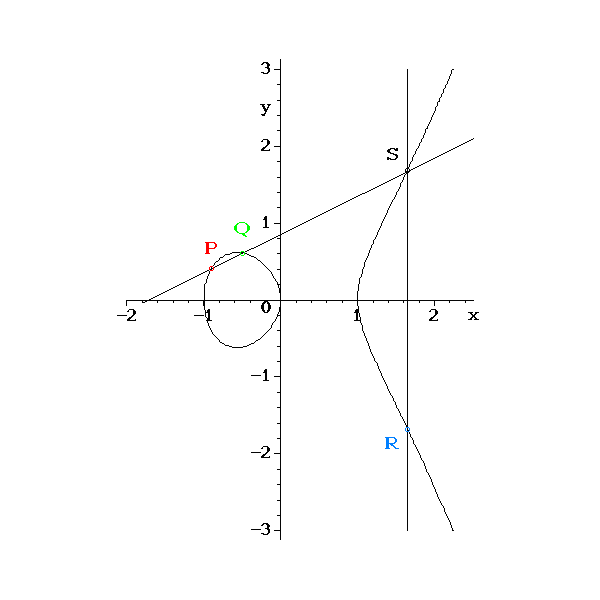
\includegraphics[scale=0.5]{../Figures/addition.png}
	\caption{The chord-tangent composition law on an elliptic curve}
	\label{chord-tangent}
\end{figure}
The addition rests upon the so-called `chord-tangent~law', which is illustrated in \cref{chord-tangent}.
% chord tangent example?
Since an elliptic curve is cubic and regular, by definition, every line intersects it with multiplicity exactly three.
This means that given two points (not necessarily distinct), the line on which those points lie (or the tangent line to the curve at the point, if the points are the same) will intersect the curve in exactly one other place.
The idea of the chord-tangent law is that we can take any two points $P$ and $Q$ and define $P * Q$ to be this third point of intersection.
Note that, for the group to be an identity, we need an element $0$ such that $0 * 0 = 0$.
For the chord-tangent law, this just means that the tangent line at $0$ intersects there with multiplicity 3, which just means that $0$ is a flex of $E$.

However, the chord-tangent~law alone is not enough to turn $E$ into a group, since associativity is not satisfied.
This can be remedied, though, by defining the elliptic curve addition law as follows.
\begin{theorem}
	For points $P$, $Q$ and $R$ on an elliptic curve with a flex $\pai$, the addition law $+$ defined by
	$$P + Q = \pai * (P * Q)$$
	turns the curve into an abelian group, where $*$ is the chord-tangent~law as defined earlier.
	The flex $\pai$ acts as the identity element of the group.
\end{theorem}
This is known as Poincaré's theorem.
\subsubsection{Canonical Forms of Elliptic Curves}
As we have introduced them so far, elliptic curves have no specific form, other than being defined by a homegeneous polynomial of degree three.
The following theorem is useful when working with elliptic curves.
\begin{theorem}
	For any elliptic curve given by a polynomial $F$, there exist projective transformations which put $F$ into one of the following forms:
	\begin{itemize}
		\item $Y^2Z - G(X,Z) = 0$ where $G(X,Z) = X^3 + aX^2Z + bXZ^2 + cZ^3$
		\item $Y^2Z - G(X,Z) = 0$ where $G(X,Z) = 4X^3 - pXZ^2 - qZ^3$
	\end{itemize}
	In either form, the curve is regular if and only if $g(x)$ (the dehomogenisation of $G(X,Z)$) has no repeated roots.
	The point $\pai = [0,1,0]$ is the unique point at infinity on the curve, and is a flex.
	The line at infinity $Z = 0$ is tangent to $F$ at $\pai$.
\end{theorem}
When dehomogenising these forms, notice that we have the affine curves $y^2 = x^3 + ax^2z + bxz^2 + cz^3$ and $y^2 = 4x^3 - pxz^2 - qz^3$.
Since $\pai = [0,1,0]$ acts as the identity on curves of this form, the elliptic curve addition law is sometimes stated as $P + Q$ equals the reflection of $P * Q$ in the $x$-axis.
